%! Author = michal
%! Date = 6/2/20

\section{TCP and QUIC Benchmarks}
\label{sec:tcp-quic-benchmarks}

We compare TCP and QUIC protocols be executing simple HTTP GET request to
https://quic.tech:8443/ address.
Under this URL is hosted server which can handle both TCP and QUIC requests.

\subsection{Benchmarks}
\label{subsec:benchmarks}
Following benchmarks were performed:
\begin{itemize}
    \item overall request time
    \item connection establishment time
    \item number of TCP/UDP packets sent
    \item overall size of UDP datagrams and TCP segments sent
\end{itemize}

\subsection{Environment}
\label{subsec:environment}
Network bandwidth:
\begin{itemize}
    \item Download: 77 Mb/s
    \item Upload: 7.7 Mb/s
    \item Ping (Wysiadłów to Warsaw): 25 ms
\end{itemize}

\subsection{Code}
\label{subsec:code}

\subsubsection{TCP and HTTP/2}
Code implementing request with TCP was written using \texttt{curl-rust}~\cite{curl-rust}
which provides Rust bindings for libcurl library~\cite{curl}.

\subsubsection{QUIC and HTTP/3}
Code implementing request with QUIC was taken from examples section
of cloudflare github repository~\cite{quiche}.

\subsection{Wireshark}
\label{subsec:wireshark}
This subsection presents example wireshark dumps from executing request with TCP and QUIC.

\begin{figure}[h]
    \centering
    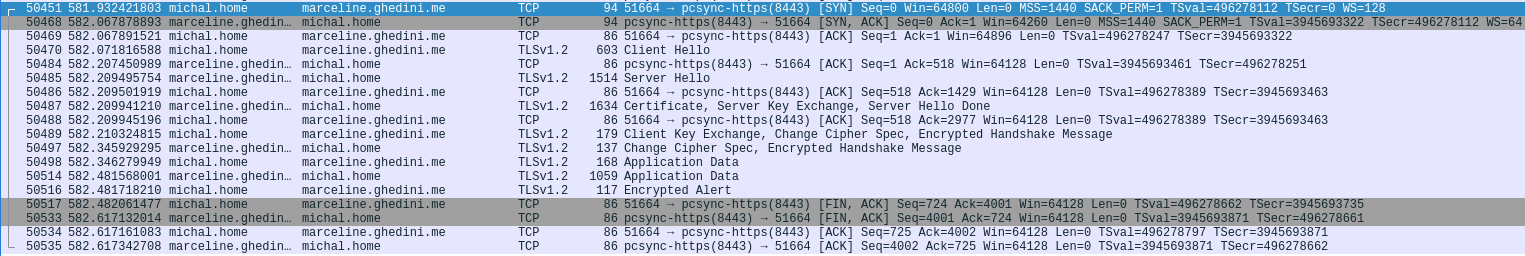
\includegraphics[width=\textwidth]{img/tcp-req-wireshark.png}
    \caption{Example wireshark dump from TCP GET request}
\end{figure}

\begin{figure}[h]
    \centering
    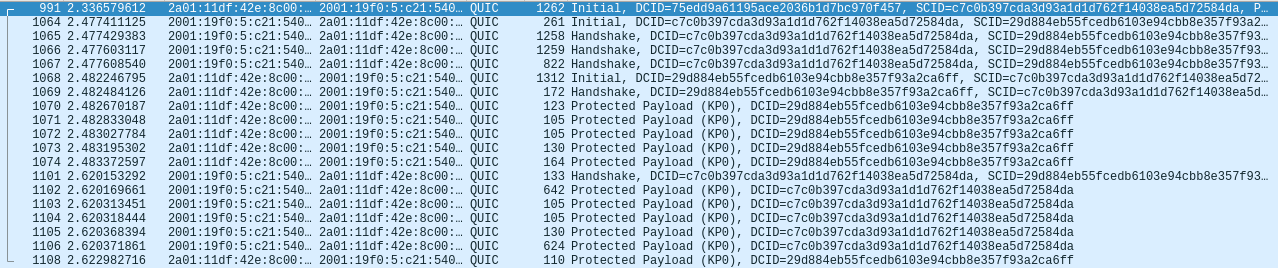
\includegraphics[width=\textwidth]{img/quic-req-wireshark.png}
    \caption{Example wireshark dump from QUIC GET request}
\end{figure}

\subsection{Results}

\begin{figure}
    \centering
    \begin{tikzpicture}
    \begin{axis}[
        xlabel=Request No.,
        ylabel=Time (s),
        legend pos = outer north east]
        \addplot table[mark=*, x index=0, y index=1] {data/time.dat};
        \addplot table[mark=*, x index=0, y index=2] {data/time.dat};
        \legend{tcp, quic}
    \end{axis}
\end{tikzpicture}

    \caption{Overall http GET request time with connection fin in case of TCP}
    \label{fig:time}
\end{figure}

\begin{figure}
    \centering
    \begin{tikzpicture}
    \begin{axis}[
        xlabel=Request No.,
        ylabel=Time (s),
        legend pos = outer north east]
        \addplot table[mark=*, x index=0, y index=1] {data/conn-est-time.dat};
        \addplot table[mark=*, x index=0, y index=2] {data/conn-est-time.dat};
        \legend{tcp, quic}
    \end{axis}
\end{tikzpicture}

    \caption{Connection establishing time}
    \label{fig:conn-est-time}
\end{figure}

\begin{figure}
    \centering
    \begin{tikzpicture}
    \begin{axis}[
%        bar width=1cm,
        enlarge x limits=1,
        ybar,
        xtick=data,
        xticklabels from table={data/packets.dat}{proto},
        legend pos = outer north east]
        \addplot table[mark=*, x expr=\coordindex, y index=3] {data/packets.dat};
        \addplot table[mark=*, x expr=\coordindex, y index=2] {data/packets.dat};
        \addplot table[mark=*, x expr=\coordindex, y index=1] {data/packets.dat};
        \legend{conn-est-packets, all-packets, all-packets-kbytes}
    \end{axis}
\end{tikzpicture}

    \caption{Packets summary}
    \label{fig:packets-summary}
\end{figure}
